\documentclass[12pt]{article}

\title{Virtual Synthesizer Development in C++}
\date{May 27th, 2024}

% author hijacking is so real https://tex.stackexchange.com/questions/63384/add-additional-text-on-title-page
\author{\parbox{\linewidth}{\centering%
	Will Sieber
	\endgraf\bigskip
	Department of Computer Science, The College of Wooster
	\bigskip
}}

\usepackage[left=1in,right=1in,top=1in,bottom=1in]{geometry}
\usepackage{amsmath}
\usepackage{hyperref}
\usepackage{setspace}
\usepackage{tikz-cd}
\usepackage{pgfplots}
\usepackage{graphicx}
\usepackage{listings}
\usepackage{wrapfig}

\graphicspath{ {./images/} }

\spacing{1.5}

\begin{document}
\maketitle

% Latex can automatically build a table of contents for you
\newpage
\tableofcontents
\newpage

\section{Abstract}
Virtual synthesizers are tools used by musicians to generate sound for use in digital audio workstations. They are repackaged dynamic-link libraries under one of several existing specifications that ensure they are compatible with host applications. Several software development kits and libraries exist with the purpose of developing these tools, but this paper will focus on development under Steinberg's Virtual Studio Technology (VST3) specification. This will serve as a quick-start guide to those interested in real time audio processing by first providing the theory behind computer audio, and then using this knowledge in a practical setting by developing a virtual additive synthesizer under the VST3 specification. This synthesizer will be able to generate several different waveforms with two different oscillators, alongside an envelope generator to control the articulation of the resulting waveform. Additional functionality common to other synthesizers will be included and discussed, but are not required to develop a functional program.
\newpage

\section{Introduction}

\subsection{Project Goals}
This project initially had one goal in mind: create sound. In order to do so, one must first process MIDI data, generate the desired waveform, and then create the user interface while ensuring the program's state changes accordingly. Upon overcoming this hurdle, several additional features can be implemented on this foundation that include additional oscillators, envelope generators, and more. Maintaining good practice while coding was an additional goal, so that others may take this project and change or modify it to their needs. With these goals in mind, the following section provides background information important to understanding what a synthesizer is, and how each component of a synthesizer work. 

\section{Synthesizer Basics}

\subsection{What is a Synthesizer?}
In essence, a synthesizer is a musical instrument that generates waveforms and provides several parameters to alter them in interesting ways. These parameters can interact with one another to create complex timbres. Development of the modern synthesizer can be traced to the late 1950s, where the Columbia-Princeton Electronic Music Center became the prime location for composers interested in new and developing technologies \cite{Pejrolo_2017}. By the 1960s, physicist Robert "Bob" Moog would create an instrument known as the "Modular" which utilized a keyboard interface, exactly like one would play on a piano or organ, which became the first (realistic) commercially available option to buyers \cite{Pejrolo_2017}. Nowadays, computers are capable of creating sound exactly like a synthesizer would, and musicians commonly use these virtual synthesizers to produce popular music. 

\subsection{Components}
There are several components of a synthesizer that work together in order to generate sound. This section will cover in detail the specific components that were implemented in software. Following this section, there will be another that provides additional components that are commonly found in other synthesizers.

\subsubsection{Oscillators}
Oscillators can be generally broken into two categories: tone generators and controllers. To generate sound, tone generators repeat periodic waves that can be expressed as mathematical expressions, such as \(f(x) = sin(x)\). More complex tone generators allow for any waveform to be repeated, regardless if they can be easily expressed as a single expression, but are not necessary to create the "fundamental" synthesizer waveforms. They also allow for a number of different waveforms to be represented in a single table, allowing for a user to select any number of waveforms in real time. For the purposes of this project, simple oscillators are used as tone generators. Controller oscillators, on the other hand, are much lower frequency than tone oscillators, and are used to control other parameters of a synthesizer. These will be discussed in brief at a later section.

There are four simple waveforms that are considered "fundamental" for a synthesizer. These are the oscillator's \textit{sine}, \textit{square}, \textit{sawtooth}, and \textit{triangle} waveforms. Each have their own characteristics distinguishing them from one another, but can be loosely described in the following ways:

\begin{enumerate}
	\item Sine waves are considered "pure", as they contain no overtones. Should every instrument be isolated to its fundamental frequency, this is the tone that would result. For this reason, one might find this waveform in the bass of a song, as more complex timbres may cause things to sound "muddy".
	\item Square waves are "hollow" and are commonly used in subtractive synthesis. They contain several frequencies above its fundamental frequency (these are known as harmonics), but not as many as sawtooth waves. Square waves can be generalized as a specific case of \textit{pulse} waveforms, where in this case the positive portion of the waveform is equal length to the negative.
	\item Sawtooth waves are "buzzy". They contain a greater number of harmonics than square waves, and are commonly used in subtractive synthesis as well.
	\item Triangle waves are not as harsh than sawtooth waves, but not as "hollow" as square waves. They contain a different set of harmonics as square waves, thus providing a different timbre.
\end{enumerate}

Images of each waveform can be seen below:

\begin{figure}[h]
	\centering
	\includegraphics[scale=0.25]{Waveforms.png}
	\caption{A diagram of sine, square, triangle, and sawtooth waveforms.}
\end{figure}

With these waveforms, musicians are capable of creating a number of sounds and timbres through the use of additional components.

\subsubsection{Envelope Generators}
In order to provide articulation, envelope generators describe how the amplitude of a particular sound should change over time. Several parameters are used to accomplish this goal, and those are the synthesizer's \textit{attack}, \textit{decay}, \textit{sustain}, and \textit{release} \cite{Pirkle_2021}. \textit{Attack} describes how much time it takes for the synthesizer to reach full amplitude upon receiving the signal to generate sound. A short attack will reach full amplitude quickly, such as playing on a piano or organ. Longer attacks will take more time to reach full amplitude, which create a "swelling" effect that is similar to that of a violin increasing in volume. \textit{Decay} describes how much time the synthesizer should take to reach a particular amplitude once the attack is finished. A longer decay will prolong a sound prior to the sustain, and vice versa. \textit{Sustain}, unlike attack and decay, describes the amplitude itself to which the decay will reach upon completion. When reached, the synthesizer will continuously play at this amplitude until a signal is sent that it should stop generating sound. Upon this signal, \textit{release} describes how long the synthesizer should take to stop generating sound by gradually decreasing the amplitude to zero. 

In more technical terms, the envelope generator of our synthesizer is its own finite state machine that modifies our signal. The signal is modified through multiplying our source to a constantly changing value. This value has different behavior as to how it changes depending on the current state, such as the attack state, the decay state, and so on. One may notice a problem with this - the rate at which the attack, decay, and release change amplitude itself is not described. Powerful synthesizers allow for this change to be represented as a polynomial function, but for the purposes of this project, the rate at which each parameter changes will simply be linear. 

With these two components in mind, one can create a simple synthesizer in the same manner that is described in this project. What follows are additional components found commonly in synthesizers, but are not required to be present. That being said, it is important to understand them to provide a complete picture of what synthesizers are capable of. 

\subsection{Extra Components}

\subsubsection*{Digitally Controlled Amplifiers}
Digitally Controlled Amplifiers (DCAs) control the final amplitude or volume of the synthesizer. A good DCA will prevent the final output signal from going beyond the range [-1, 1] thus preventing unwanted artifacts \cite{Pirkle_2015}. For the purposes of this project, volume is controlled from each source oscillator.

\subsubsection*{Low-Frequency Oscillators}
Low-Frequency Oscillators (LFOs) are generally used as an input to automate other parameters of a synthesizer, allowing for a greater range of timbres. They generally exist in a range much lower than human hearing (\textless 20 Hz) and usually consist of the same basic waveforms that tone generator oscillators use (sine, square, sawtooth, and triangle).

\subsubsection*{Filters}
Filters are a form of subtractive synthesis that remove frequencies based on a particular \textit{cutoff}. There are several types of filters that exist, with the most common being \textit{lowpass}, \textit{highpass}, and \textit{bandpass}. Lowpass filters remove higher frequencies, allowing lower frequencies to "pass through" the filter, resulting in a "dark" sound. Highpass filters do the opposite, removing lower frequencies and passing through higher ones based on a particular cutoff frequency. Bandpass filters remove both upper and lower frequencies from a particular cutoff.

\newpage
\section{Theory}

There are a number of problems one faces when attempting to process real time audio. They can be summed up by asking the following questions:

\begin{enumerate}
	\item "How do we create a digital representation of sound?"
	\item "How do we process audio fast enough to ensure there are no unwanted artifacts in our software?"
\end{enumerate}

The following section will address these concerns and provide the theory of what is occurring in the background of our software.

\subsection{Discrete Signals}
Sound is represented digitally by taking samples of the original source. An audio sample measures the amplitude of the source wave at a point in time, which is represented in code as a floating point number in the range \([-1, 1]\) \cite{Doumler}. Given a piece of audio, the number of samples per second represent the \textit{sample rate} of our recording. As a result, a higher sample rate will result in audio that more closely resembles the original source. Consider the following sine wave:

\begin{figure}[h] % [h] used to prevent {figure} from doing weird positioning
\begin{center}
	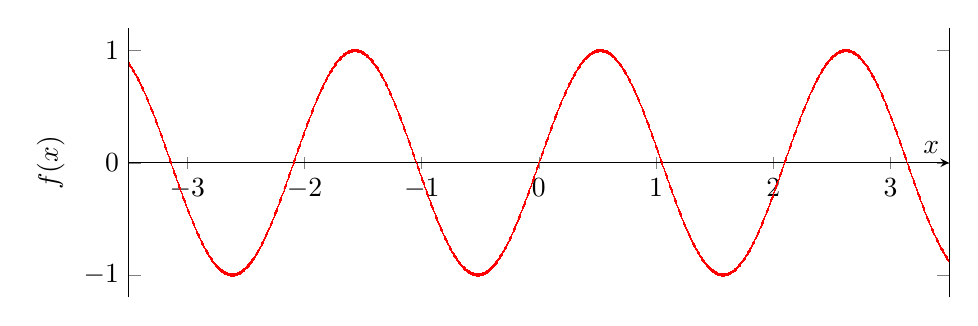
\begin{tikzpicture}
		\begin{axis} [
			axis x line = middle, % The x axis should go through the origin
			xlabel = \(x\),
			ylabel = {\(f(x)\)},
			height = 5cm,
			width = 12cm
			]
			
			\addplot [
			jump mark mid,
			domain = -3.5:3.5,
			samples = 1000,
			very thick, red
			] {(sin(deg(3 * x)))};
			
		\end{axis}
	\end{tikzpicture}
	\caption{A graph of the sine wave \(f(x) = sin(3x)\).}
\end{center}
\end{figure}

\newpage

A computer would interpret this signal by taking a number of samples at regular intervals:

\begin{figure}[h] % [h] used to prevent {figure} from doing weird positioning
	\begin{center}
		\begin{tikzpicture}
			\begin{axis} [
				axis x line = middle, % The x axis should go through the origin
				xlabel = \(x\),
				ylabel = {\(f(x)\)},
				height = 5cm,
				width = 12cm
				]
				
				\addplot+ [
				ycomb,
				mark = text,
				text mark = , % so jank
				domain = -3.5:3.5,
				samples = 40,
				red
				] {(sin(deg(3 * x)))};
				
			\end{axis}
		\end{tikzpicture}
		\caption{A discrete graph of the sine wave \(f(x) = sin(3x)\) taken with 40 samples.}
	\end{center}
\end{figure}

Thus, the higher number of samples per second would result in a sound that more closely resembles Figure 2:

\begin{figure}[h] % [h] used to prevent {figure} from doing weird positioning
	\begin{center}
		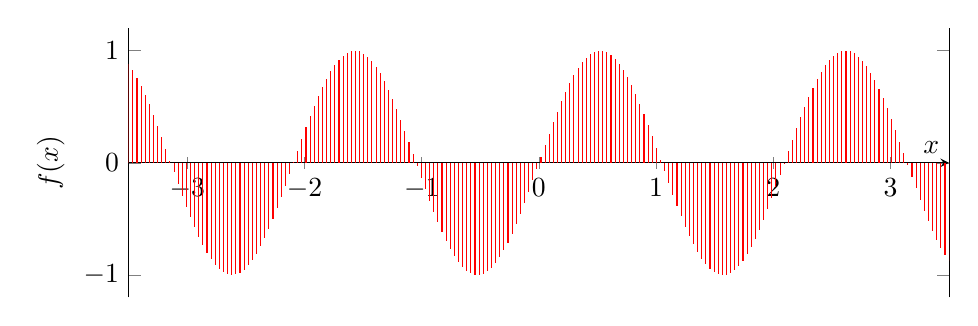
\begin{tikzpicture}
			\begin{axis} [
				axis x line = middle, % The x axis should go through the origin
				xlabel = \(x\),
				ylabel = {\(f(x)\)},
				height = 5cm,
				width = 12cm
				]
				
				\addplot+ [
				ycomb,
				mark = text,
				text mark = , % so jank
				domain = -3.5:3.5,
				samples = 200,
				red
				] {(sin(deg(3 * x)))};
				
			\end{axis}
		\end{tikzpicture}
		\caption{A discrete graph of the sine wave \(f(x) = sin(3x)\) taken with 200 samples.}
	\end{center}
\end{figure}


Most commonly, audio files will have a sample rate of 44.1 kHz or 48 kHz. That means our software will need to process that number of samples per second, continuously \cite{Doumler}. For the purposes of this project, there are two audio sources: \textit{OSC1} and \textit{OSC2}. Each oscillator will generate a sound sampled at the rate that is decided by the host application.

\subsection{Buffers}
When processing, there are a stack of processes that one's audio information must traverse before it is played on the system's speakers. Section 4.3 describes this stack. At regular intervals, a system's integrated sound card requests audio data to be sent to the system's speakers. This request does not wait for anything. \cite{Doumler} As such, it would be incredibly inefficient for this call to be done for every single audio sample, so to process this large amount of data quickly, \textit{buffers} are used. 

A buffer is an array of audio samples, with a length decided by the programmer. Should one use a smaller sized array as a buffer, a higher number of calls would be required to meet the specified 44.1 or 48 kHz output. This does have the benefit of feeling lower-latency, but at the cost of being more computationally expensive \cite{Doumler}. Should one exceed the time limit that one has to process a particular waveform, each subsequent buffer will be delayed, causing unwanted popping and clipping in the audio output \cite{Goodlife}.  

\subsection{Flow of Information}

% the goat https://ctan.math.washington.edu/tex-archive/graphics/pgf/contrib/tikz-cd/tikz-cd-doc.pdf
% i am just gonna put an image here
\begin{center}
	\begin{figure}[h]
		\includegraphics[scale=0.4]{image1.png}
		\caption{A graph of how audio information is handled throughout the system.}
	\end{figure}
\end{center}

That being said, there is no reason that buffers should miss the provided time limit, as computers have become increasingly efficient, assuming one maintains proper programming conventions. For example, printing text to the terminal while performing calculations can cause a buffer to be missed. Operating system calls take a significant amount of time relative to what is allowed for by the audio driver, so it is best to avoid them altogether \cite{Doumler}.

This extends into using unfamiliar classes and functions that may be present in 3rd party libraries, should one use them alongside a VST application. Common practice says to "use what you trust", and to create your own functions should you be unsure \cite{Goodlife}.

\newpage
\section{Implementation using VST3 SDK}

\subsection{Development Tools}
The VST3 SDK contains several tools and programs that assist in developing the boilerplate code necessary for creating VST applications and ensuring they fall under the required specification. These are the project generator, GUI editor, and validator. By using the project generator, a CMakeLists text file is generated, as well as a Visual Studio solution pre-configured with several components to test VST applications easily. 

Utilizing a CMake C++ project for development is effective. However, it does need to be changed frequently should additional files be added or changed (such as additional header files or custom graphics). A GUI-specific file \textit{myplugineditor.uidesc} must be correctly located in \verb*|resource/myplugineditor.uidesc|, or else undefined behavior will occur when attempting to load the GUI of the VST.

There are two solution configurations included with the generated file: \verb*|Debug| and \verb*|Release|. When the Visual Studio solution is started, a host application launches that can quickly test MIDI input and audio output. Both configurations create a .vst3 file that can be launched with any digital audio workstation, but \verb*|Debug| allows for changes to be made to the GUI from the GUI editor.

Lastly, when programming, functions and classes under the VST3 SDK are organized under namespaces, in order to avoid name collisions \cite{Pirkle_2015}. The Steinberg namespace contains the Vst namespace, which in turn contains the programmer's namespace created by the project generator. 

Now that one can begin development, obtaining MIDI input is necessary before one can generate waveforms at the correct frequency. 

\subsection{Obtaining MIDI Input}
Every MIDI note corresponds to a particular integer \textit{n} in the range of 21 to 108. The corresponding note names range from A0 - C8, which in turn provides a range of frequencies between 27.5 Hz to 4186 Hz \cite{MIDI_online}. By utilizing a reference pitch, one can calculate the frequency \textit{F} from a particular MIDI note \textit{n} using the following equation:

$$ F_n = 440 * 2^{(n - 69) / 12} $$

In this case, the reference pitch is A4 at 440 Hz, with the corresponding MIDI number 69. A graph of each MIDI note and their corresponding frequency can be found on Figure 6.

% cool graphix https://tex.stackexchange.com/questions/55161/how-to-arrange-image-and-text-to-appear-side-by-side
\begin{wrapfigure}[20]{r}{5.5cm}
	\includegraphics[width=5.25cm]{notes.png}
	\caption{A graph of MIDI notes and their frequencies \cite{MIDI_online}.}\label{wrap-fig:1}
\end{wrapfigure} 

For MIDI notes lower than the reference note A4, the reference pitch is multiplied by 2, to the power of a negative number. While this may seem incorrect at first glance, this is indeed expected behavior as the resulting frequency will be one that is \textit{below} the initial reference pitch. From this, one is able to obtain the correct frequency upon receiving a particular MIDI signal.

The VST3 SDK contains an event-handling class under the \verb*|Steinberg::Vst| namespace. When checking for a \verb|kNoteOnEvent| signal, one can obtain the MIDI note ID by using \verb*|event.noteOn.pitch|. From here, it is simply a matter of using the equation above and correctly initializing any additional parameters for the oscillator. 

\subsection{Creating Oscillators}
Upon receiving MIDI input, one can begin generating waveforms of a particular type. For this synthesizer, these will consist of the four previously mentioned waveforms: sine, square, sawtooth, and triangle. To begin, a \textit{for} loop is utilized to step through each sample of a buffer. In the VST SDK, the \verb*|&data| parameter located in \verb*|Steinberg::Vst::ProcessData| contains the specific value \textit{numSamples} which has the buffer size. Using this, one then checks the state at which the GUI is currently in to determine which waveform to generate.

Generating a sine wave is as simple as using the \verb*|sin()| function provided with C++. By providing the phase of our wave as an input and multiplying it by our current oscillator amplitude, one generates a sine wave:

\begin{lstlisting}
		outL[i] = fOsc1 * sin(fOsc1Phase);
\end{lstlisting} 

The following equations generate sawtooth, square, and triangle waves, respectively:

Sawtooth:
\begin{lstlisting}
	outL[i] = fOsc1 * (1.0f - (2.0f * fOsc1Phase / TWO_PI));
\end{lstlisting} 

Square:
\begin{lstlisting}
	if (fOsc1Phase <= (TWO_PI / 2.f)) {
		outL[i] = fOsc1 * 1.0f;
	}
	else {
		outL[i] = fOsc1 * -1.0f;
	}
\end{lstlisting} 

Triangle:
\begin{lstlisting}
	double temp = -1.0f + (2.0f * fOsc1Phase / TWO_PI);
	outL[i] = fOsc1 * 2.0f * (fabs(temp) - 0.5f);
\end{lstlisting} 


\subsection{Creating An Envelope Generator}


\newpage
\section{Conclusion and Future Work}
In this paper, we discussed the fundamentals of how synthesizers work, and used this knowledge to create a virtual synthesizer utilizing the Virtual Studio Technology standard. This synthesizer obtains MIDI signals as input, and computes the frequency and waveform necessary to provide the desired output in one's host application. This signal can be further manipulated to provide articulation through the use of an envelope generator, which allows a musician to specify the attack, delay, sustain, and release of a particular sound.

As for future work, there are several routes to which one can take upon completion of this project. Should one continue working with MIDI signals as input, a more powerful wavetable synthesizer can be developed. As mentioned previously, this would allow waveforms of any type to be generated (such as by providing a wave file as input), and would have the functionality of morphing between several waveforms from a table in real time. If one would rather change gears and begin using sound itself as an input, then an \textit{effect plugin} can be created, such as one that provides reverb or chorus to a particular audio file. In both cases, several algorithms exist that each provide a slightly different sound that can be explored further by looking into different digital signal processing techniques.

\newpage
% Bibliography
\bibliography{bibliography}
\bibliographystyle{abbrv}

\end{document}